\chapter{Медиафайлы}
\label{sec:chapter_media}

В библиотеку медиафайлов можно загружать изображения, звуковые файлы, видео и файлы других типов. Какие-то файлы публикуются для просмотра и прослушивания, а другие - для скачивания.
Для просмотра медиафайлов выберите меню «Медиафайлы/Библиотека» (см. рис. \ref{fig:pic_media_library})

\begin{figure}[htp]
    \centering
	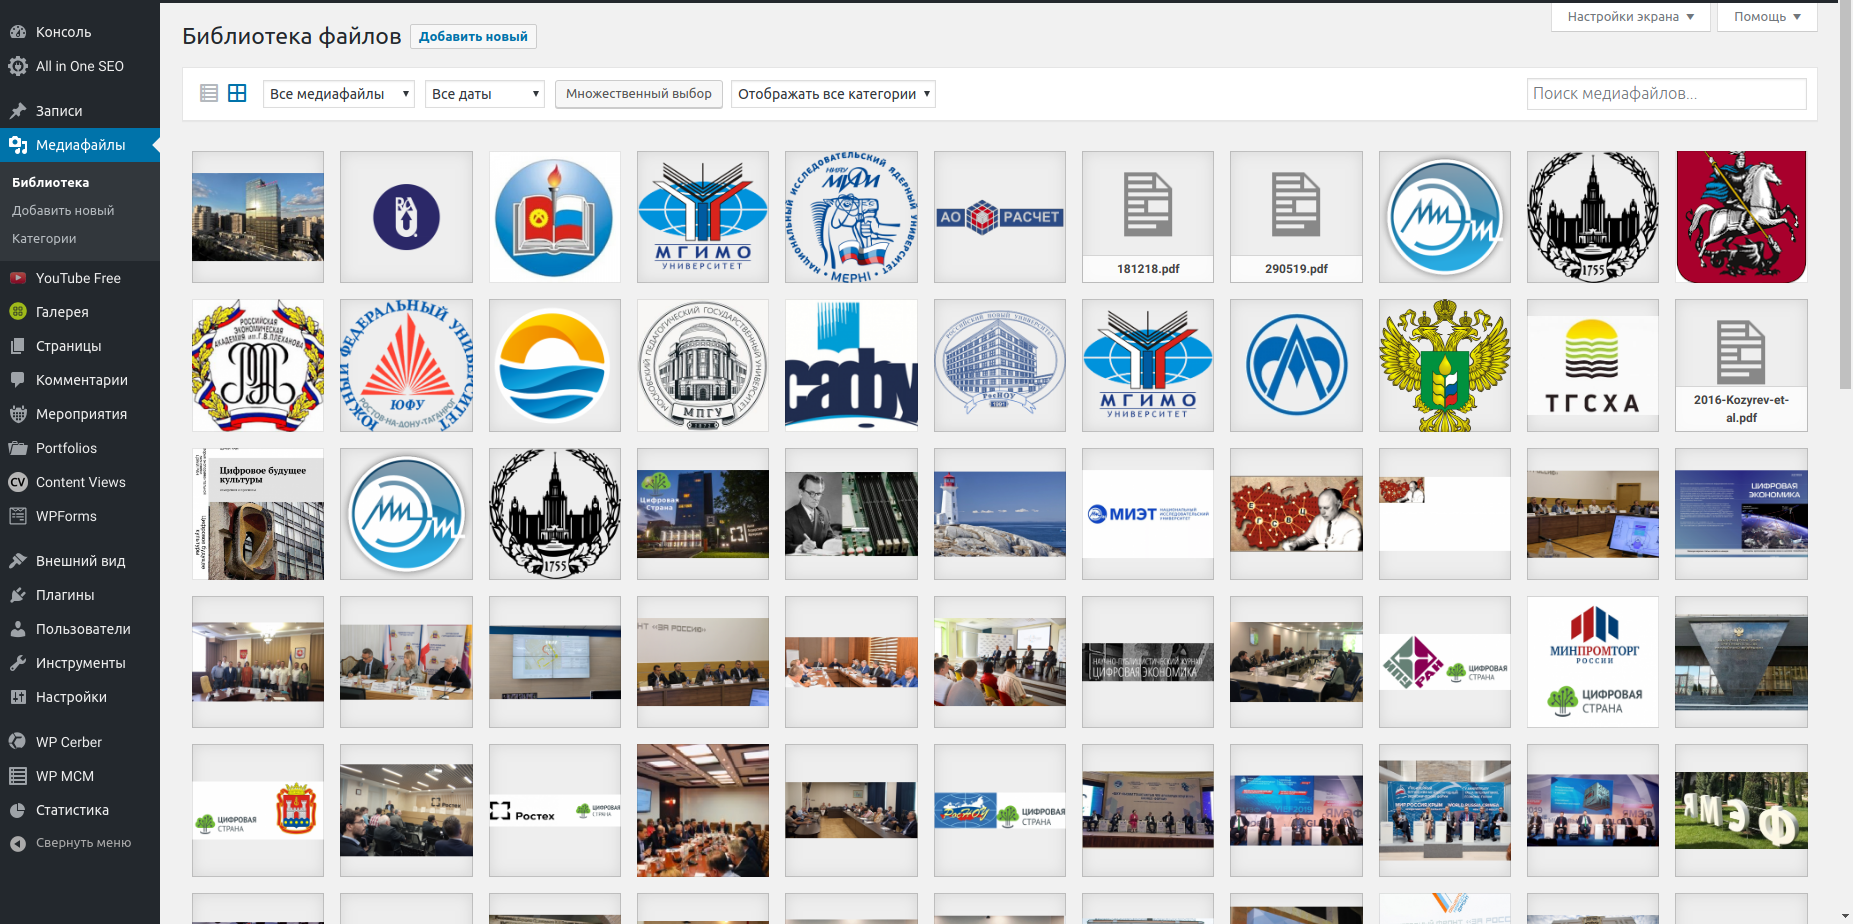
\includegraphics[width=\textwidth]{media_library.png}
    \caption{Библиотека медиафайлов}
    \label{fig:pic_media_library}
\end{figure}


\section{Категории медиафайлов}
\label{sec:part_cat_media}

Категории медиафайлов служат для удобства их поиска.
Создать или редактировать (удалить) категорию можно в разделе меню «Медиафайлы/Media Categories» (см. рис. \ref{fig:pic_media_library})

\begin{figure}[htp]
    \centering
	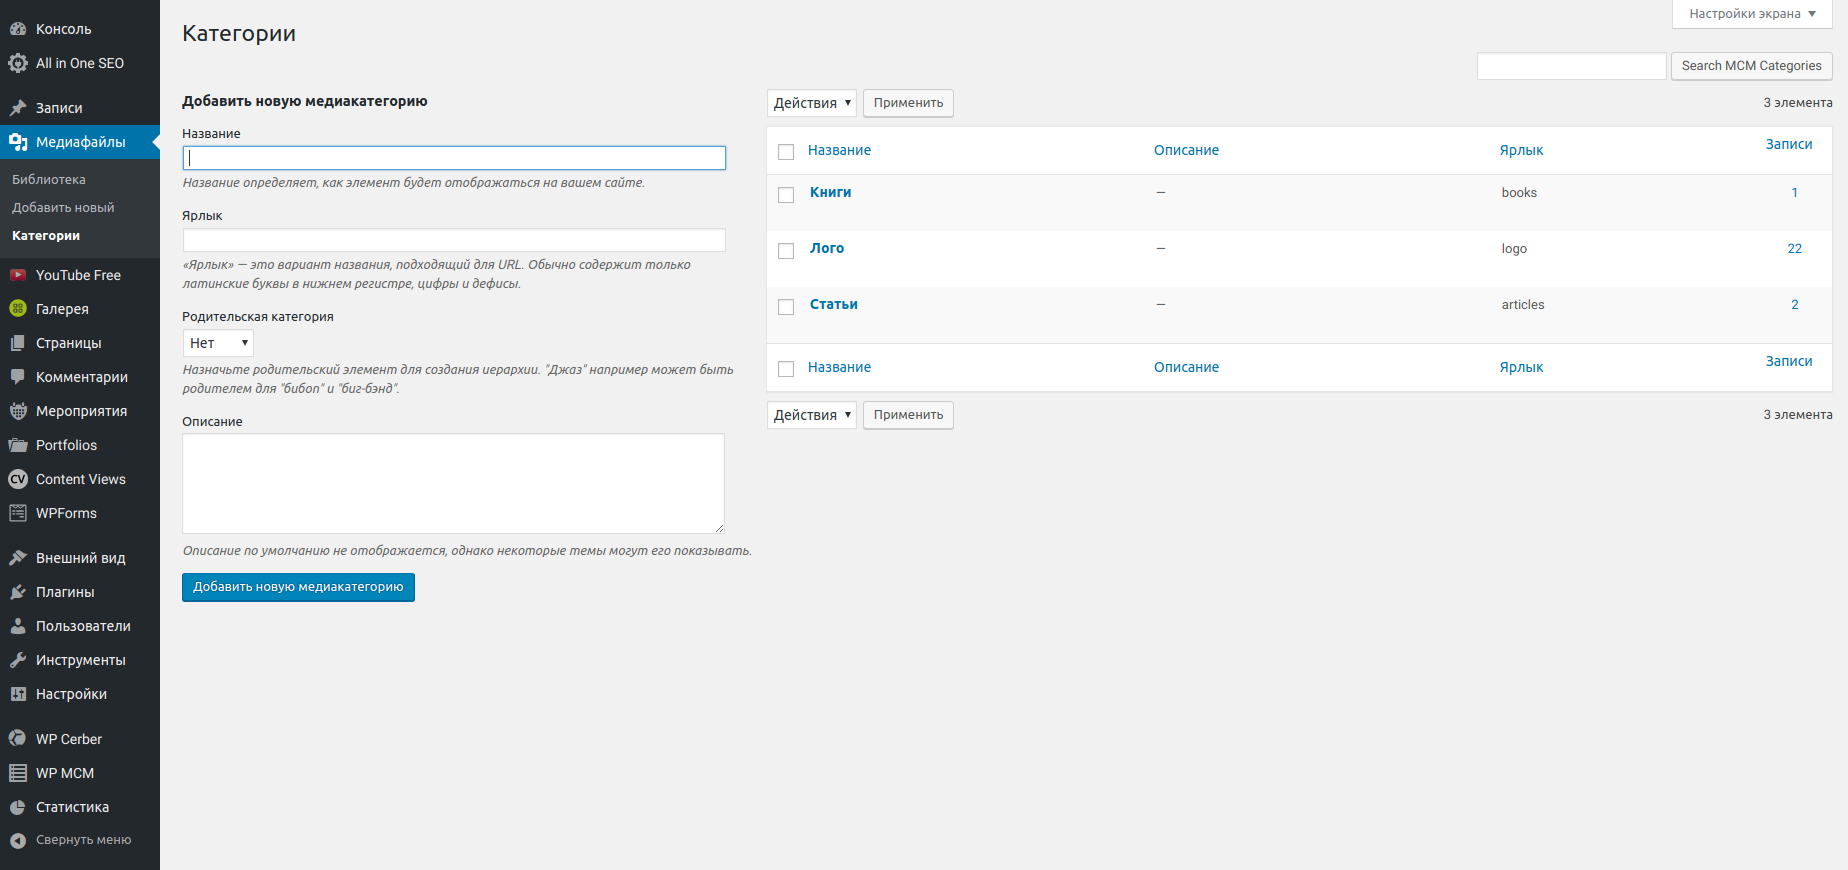
\includegraphics[width=\textwidth]{media_cat.png}
    \caption{Категории медиафайлов}
    \label{fig:pic_media_cat}
\end{figure}

\section{Загрузка медиафайлов}
\label{sec:part_upload}

На административной панели перейдите в меню «Медиафайлы/Добавить новый».
Появится страница, с которой вы можете «Загрузить новый медиафайл» или медиафайлы (см. рис. \ref{fig:pic_media_upload}).

\begin{figure}[htp]
    \centering
	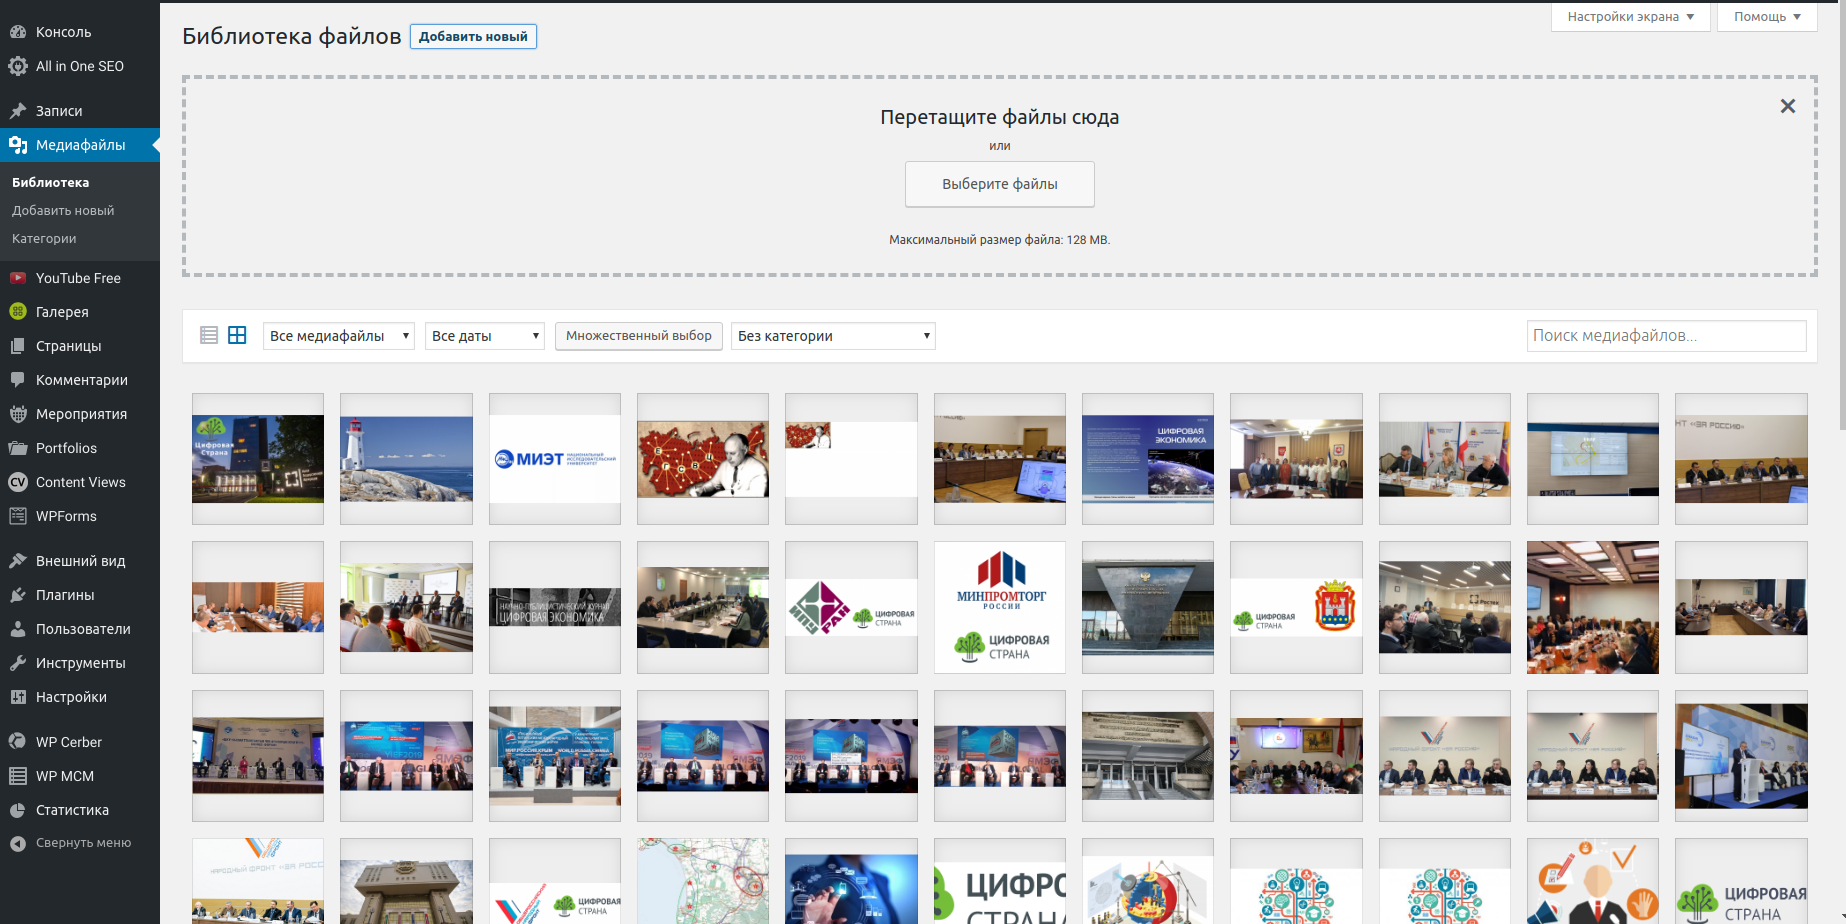
\includegraphics[width=\textwidth]{media_upload.png}
    \caption{Загрузка медиафайлов}
    \label{fig:pic_media_upload}
\end{figure}

После загрузки медиафайлов перейдите в меню «Медифайлы/Библиотека» и в раскрывающемся списке категорий выберите пункт «Без категории» (см. рис. \ref{fig:pic_media_no_cat}). Далее выберите медиафайл, появиться раздел «Media Categories» (Категории медиафайлов). Выберите категорию медиафайла.

\begin{figure}[htp]
    \centering
	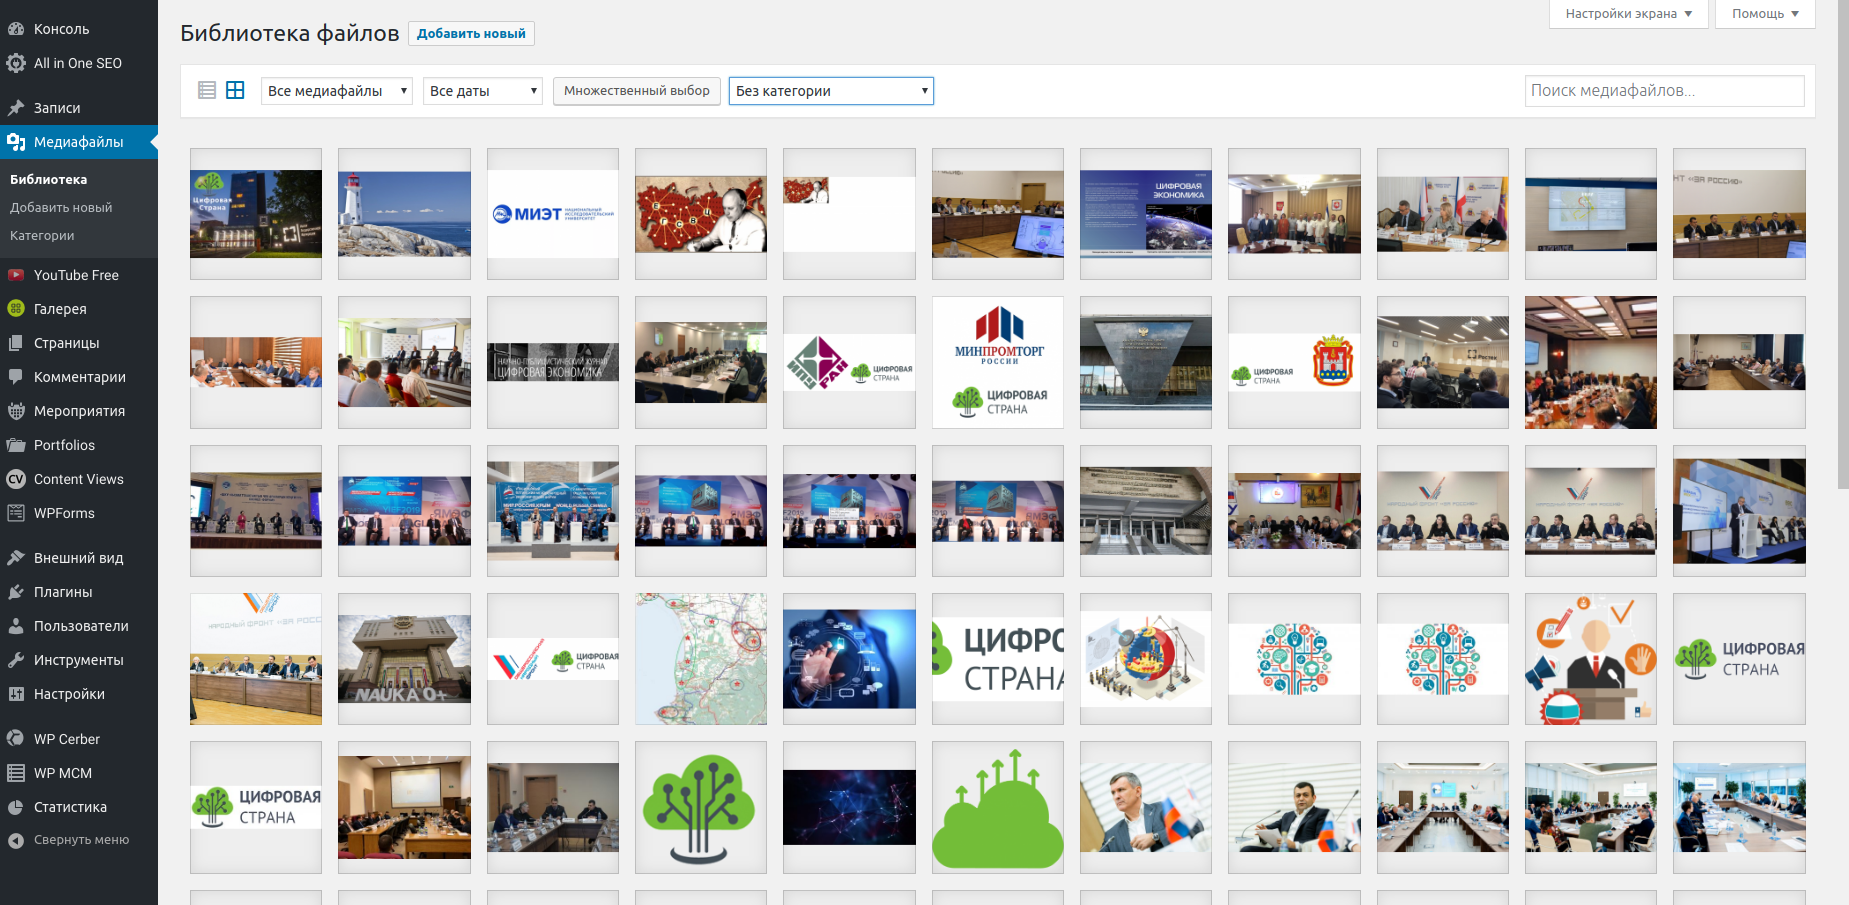
\includegraphics[width=\textwidth]{media_no_cat.png}
    \caption{Привязка медиафайла к категории}
    \label{fig:pic_media_no_cat}
\end{figure}

